\documentclass[tc_tp3_anexo_main.tex]{subfiles}

\begin{document}

\chapter{Respuesta en frecuencia del filtro low-pass}

En la figura \ref{fig:ej2_LP_bode} se observa la superposici\'on de la respuesta en frecuencia medida, calculada, y simulada. La medici\'on y la simulaci\'on est\'an tomadas con el restador, mientras que el c\'alculo considera la salida diferencial. Se observa que la simulaci\'on y el c\'alculo se separan en aproximadamente el mismo rango de frecuencia que los otros filtros. El m\'odulo de la medici\'on se diferencia del de la simulaci\'on a partir de los $100\, KHz$ y la frecuencia a partir de los $30\, KHz$. Se muestra en la figura \ref{fig:ej2_LP_bode_con_caps} la comparaci\'on entre la medici\'on y la simulaci\'on considerando una capacidad par\'asita en la entrada de los op-amps de $6pF$. Este cambio en la simulaci\'on mejora el ajuste entre $100\, KHz$ y $500\, KHz$, y predice correctamente la altura y posici\'on del sobrepico en $500\, KHz$.

\begin{figure*}[bp]
\centering
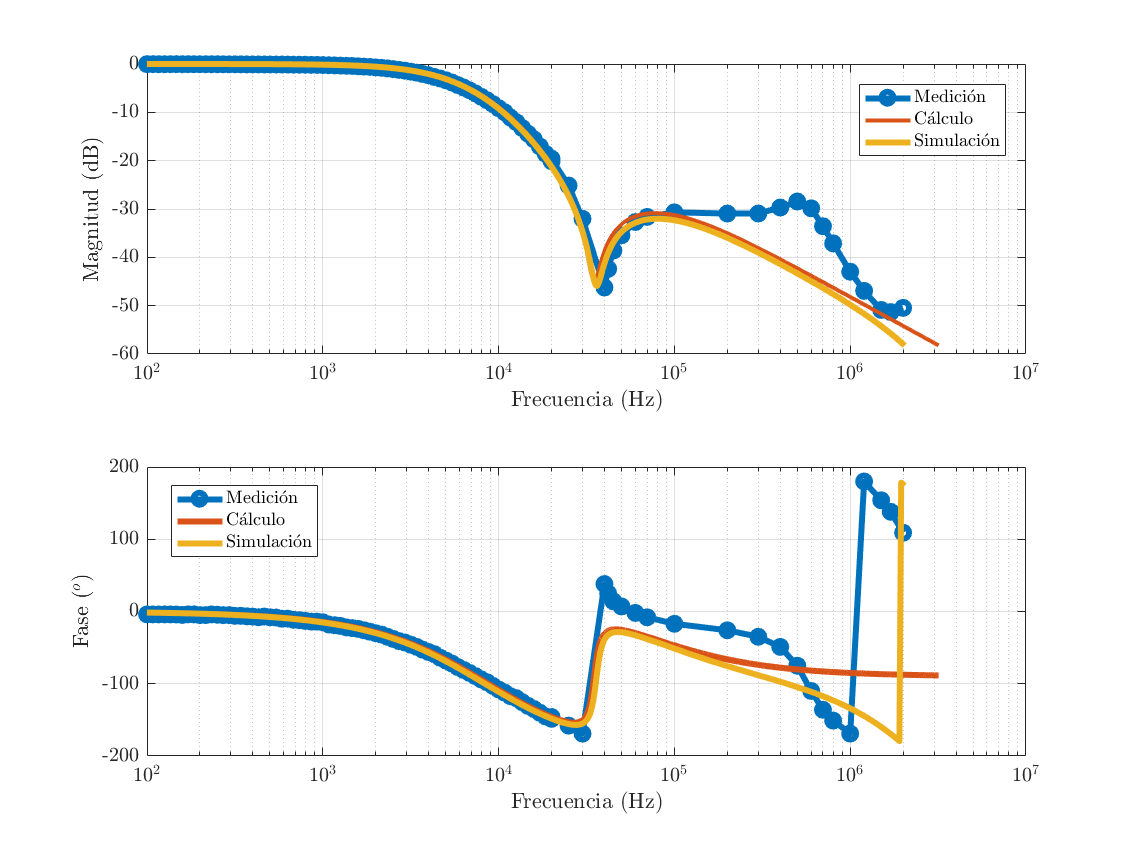
\includegraphics[width=0.7\textwidth]{imagenes/LP_bode.png}

\caption{Respuesta en frecuencia del filtro low-pass calculada, medida, y simulada}
\label{fig:ej2_LP_bode}
\end{figure*}


\begin{figure*}[bp]
\centering
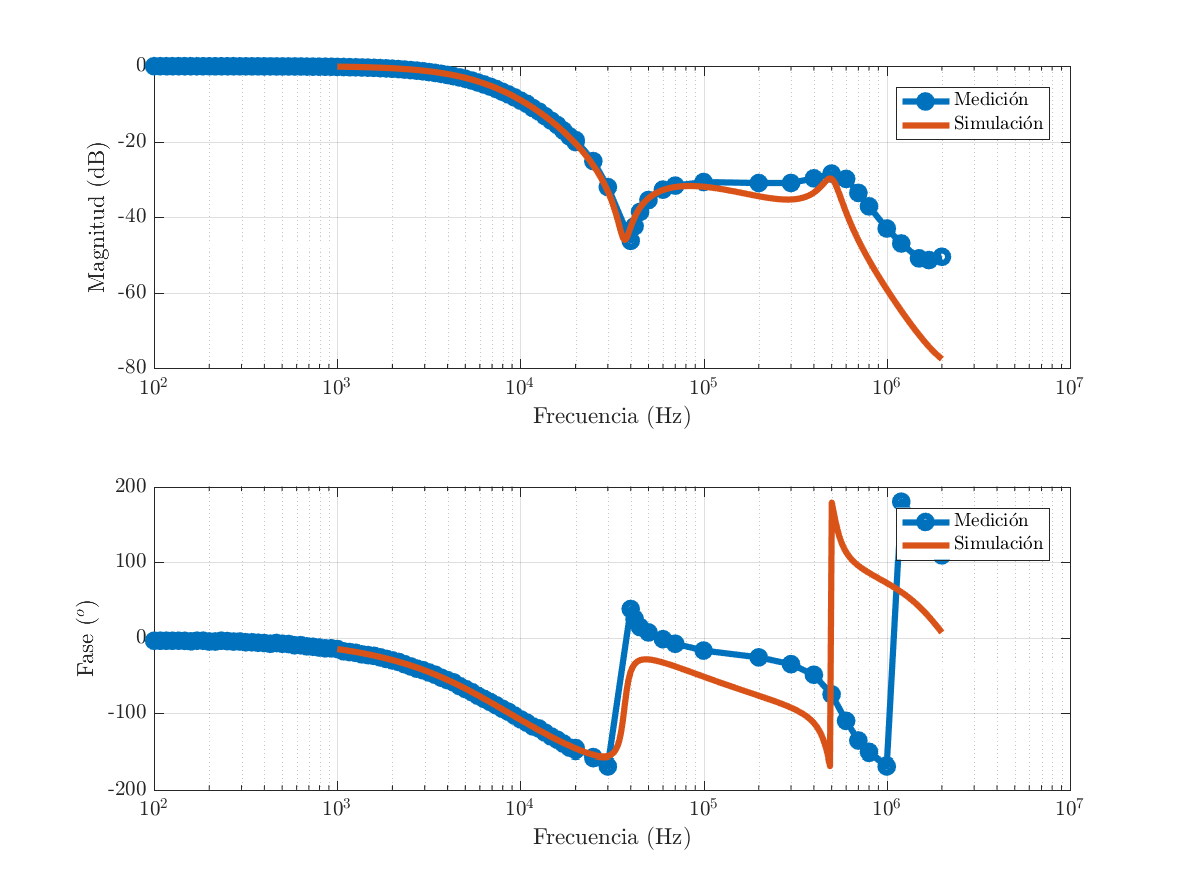
\includegraphics[width=0.7\textwidth]{imagenes/LP_bode_cap.png}

\caption{Respuesta en frecuencia del filtro low-pass medida y simulada considerando una capacidad par\'asita de $6pF$ en la entrada de los op-amps}
\label{fig:ej2_LP_bode_con_caps}
\end{figure*}


\end{document}